\begin{mainquestion}{residentialpower}{Mesh Analysis}
The DC equivalent circuit of a simple residential power distribution is shown below. $R_{w}$ represents the hot wire (typically black) resistance, and $R_{n}$ represents the neutral wire (typically white) resistance. The other resistances represent loads that are drawing power: $R_{1}$ and $R_{2}$ are loads on 120 V supplies while $R_{3}$ is a load on a 240 V appliance such as a stove or a dryer.

\begin{center}
    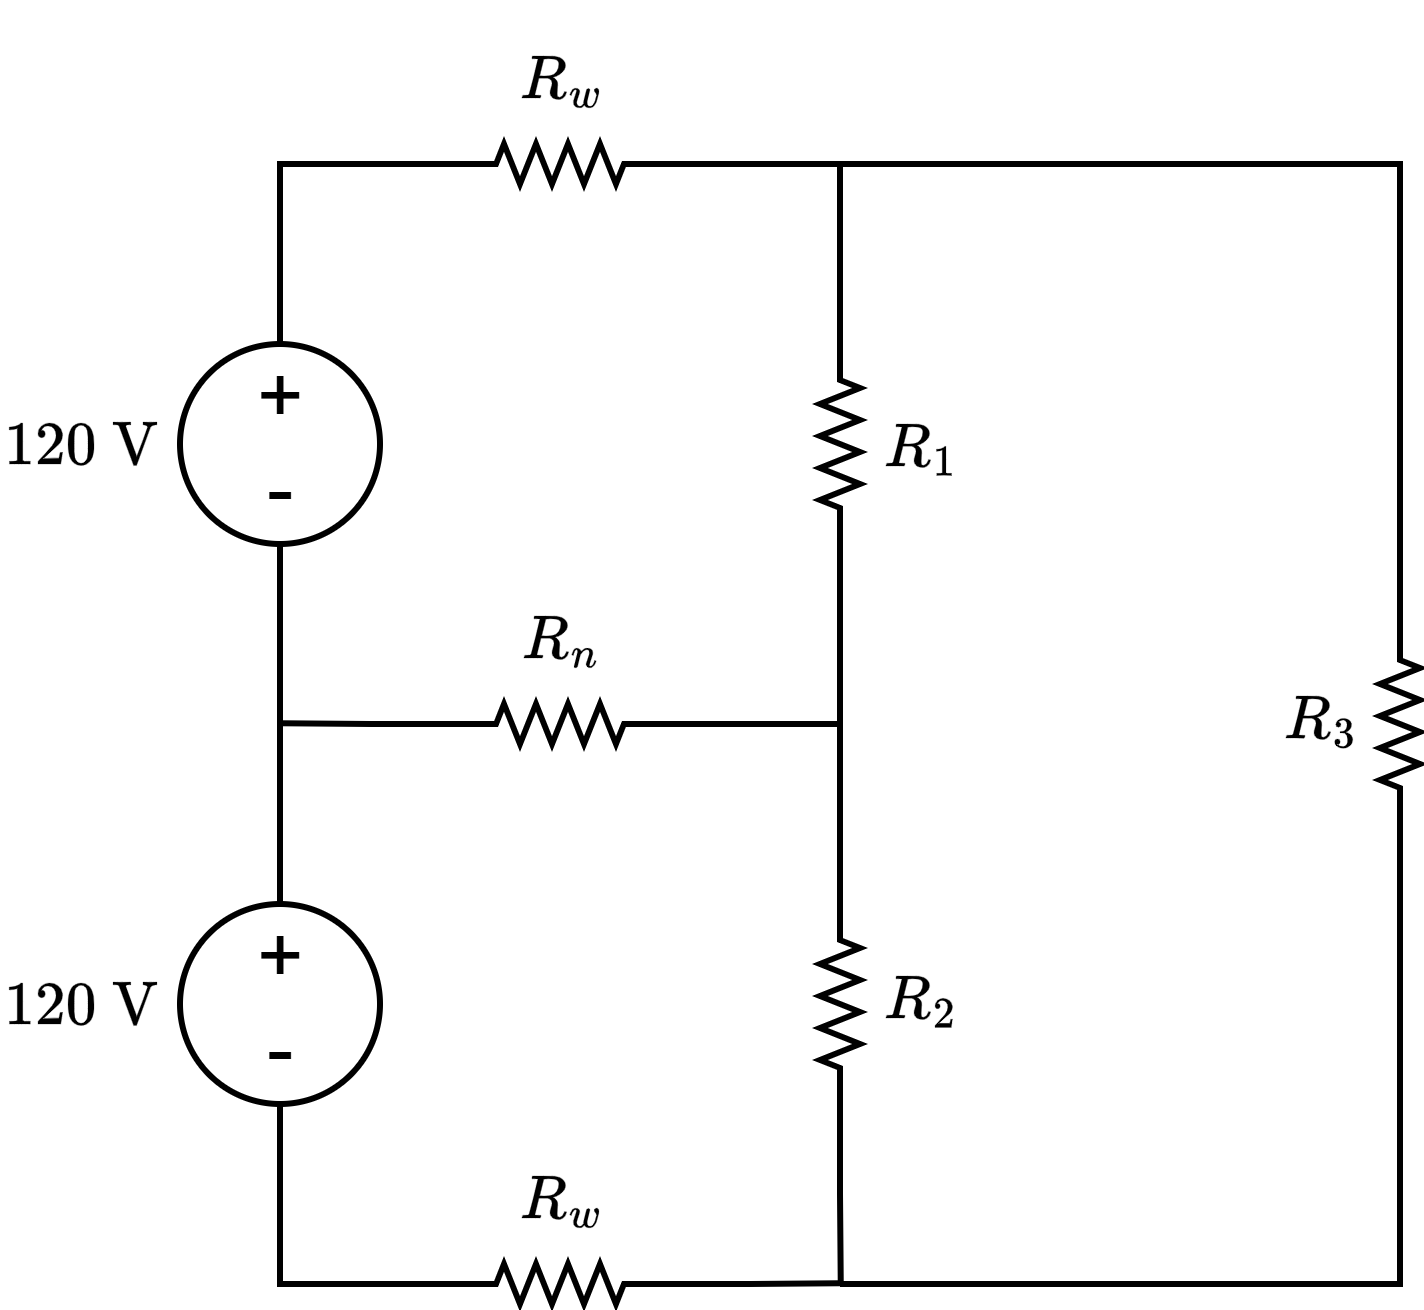
\includegraphics[width=4in]{circuit.png}
\end{center}

\begin{partquestion}{meshanalysis}{If $R_{w}=R_{n}=\qty{0.2}{\ohm}$, $R_{1}=\qty{5}{\ohm}$, $R_{2}=\qty{12}{\ohm}$, and $R_{3}=\qty{13}{\ohm}$, use mesh analysis to determine the voltage across each of the three loads.}
\begin{answer}
Create three mesh loops in the clockwise direction for the three currents $i_{1}$ in the top-left loop, $i_{2}$ in the bottom-left loop, and $i_{3}$ in the right-hand loop. Using KVL around each loop gives:

\begin{gather*}
R_w i_1 + R_1 (i_1 - i_3) + R_n (i_1 - i_2) = 120 \\
R_w i_2 + R_2 (i_2 - i_3) + R_n (i_2 - i_1) = 120 \\
R_3 i_3 + R_1 (i_3 - i_1) + R_2 (i_3 - i_2) = 0
\end{gather*}

Then we gather like terms:

\begin{gather*}
(R_w + R_1 + R_n)i_1 - R_n i_2 - R_1 i_3 = 120 \\
- R_n i_1 + (R_w + R_2 + R_n)i_2 - R_2 i_3 = 120 \\
- R_1 i_1 - R_2 i_2 + (R_1 + R_2 + R_3)i_3 = 0
\end{gather*}

And this can be neatly written as a matrix:

\[
\begin{bmatrix}
R_w + R_1 + R_n & -R_n & -R_1 \\
-R_n & R_w + R_2 + R_n & -R_2 \\
-R_1 & -R_2 & R_3 + R_1 + R_2
\end{bmatrix}
\begin{bmatrix}
i_1 \\
i_2 \\
i_3
\end{bmatrix}
=
\begin{bmatrix}
120 \\
120 \\
0
\end{bmatrix}
\]

Substituting the given values produces:

\[
\begin{bmatrix}
5.4 & -0.2 & -5 \\
-0.2 & 12.4 & -12 \\
-5 & -12 & 30
\end{bmatrix}
\begin{bmatrix}
i_1 \\
i_2 \\
i_3
\end{bmatrix}
=
\begin{bmatrix}
120 \\
120 \\
0
\end{bmatrix}
\]

Solving these equations either by hand or some matrix solver like MATLAB gives the following:
\begin{align*}
    i_1 &= \frac{315}{8} \approx \qty{39.4}{\ampere}\\
    i_2 &= \frac{435}{16} \approx \qty{27.2}{\ampere}\\
    i_3 &= \frac{279}{16} \approx \qty{17.4}{\ampere}
\end{align*}

The voltages across the three loads are then:
\begin{align*}
v_{1} &= (i_{1}-i_{3}) R_{1} = \left( \frac{315}{8} - \frac{279}{16} \right) 5 = \frac{1755}{16} = \qty{109.6875}{\volt} \\
v_{2} &= (i_{2}-i_{3}) R_{2} = \left( \frac{435}{16} - \frac{279}{16} \right) 12 = \qty{117}{\volt} \\
v_{3} &= i_{3} R_{3} = \frac{279}{16} \cdot 13 = \frac{3627}{16} = \qty{226.6875}{\volt}
\end{align*}
\end{answer}
\end{partquestion}

\begin{partquestion}{openneutral}{If a wiring fault occurs such that the neutral becomes an open circuit, recalculate the voltages across the loads.}
\begin{answer}
With the neutral open, $R_{n}\to\infty$ and the left-hand and right-hand loops remain. Let $i_{1}$ be the clockwise current in the left loop and $i_{2}$ be the clockwise current in the right loop.

The KVL system becomes:
\begin{gather*}
R_wi_1 + (R_1 + R_2)(i_1 - i_2) + R_wi_1 = 240 \\
(R_1 + R_2)(i_2 - i_1) + R_3i_2 = 0
\end{gather*}

Gather like terms:
\begin{gather*}
(2R_w + R_1 + R_2)i_1 - (R_1 + R_2)i_2 = 240 \\
- (R_1 + R_2)i_1 + (R_1 + R_2 + R_3)i_2 = 0
\end{gather*}

As a matrix:
\[
\begin{bmatrix}
2R_w + R_1 + R_2 & -R_1 -R_2\\
-R_1 -R_2 & R_1 + R_2 + R_3
\end{bmatrix}
\begin{bmatrix}
i_1 \\
i_2
\end{bmatrix}
=
\begin{bmatrix}
240 \\
0
\end{bmatrix}
\]

Substituting values yields:
\[
\begin{bmatrix}
17.4 & -17\\
-17 & 30
\end{bmatrix}
\begin{bmatrix}
i_1 \\
i_2
\end{bmatrix}
=
\begin{bmatrix}
240 \\
0
\end{bmatrix}
\]

Solving gives $i_{2} = \frac{4080}{233} \approx \qty{17.51}{\ampere}$ and $i_{1} = \frac{7200}{233} \approx \qty{30.90}{\ampere}$. The load voltages are:
\begin{align*}
v_{1} &= (i_{1}-i_{2})R_1 = \frac{15600}{233} \approx \qty{66.95}{\volt} \\
v_{2} &= (i_{1}-i_{2})R_2 = \frac{13337}{83} \approx \qty{160.69}{\volt} \\
v_{3} &= i_{2} R_3 = \frac{19577}{86} \approx \qty{227.64}{\volt}
\end{align*}
\end{answer}
\end{partquestion}

\begin{partquestion}{deviceimpact}{Postulate what might happen to a sensitive device represented by $R_{2}$ if it is plugged into this faulty circuit.}
\begin{answer}
Because $R_{2}$ now sees over 160 V instead of the expected 120 V, a sensitive device is likely to be exposed to an overvoltage condition. This can damage components, cause device failure, or lead to unsafe operation.
\end{answer}
\end{partquestion}

\end{mainquestion}
